\documentclass{beamer}
%
% Choose how your presentation looks.
%
% For more themes, color themes and font themes, see:
% http://deic.uab.es/~iblanes/beamer_gallery/index_by_theme.html
%
\mode<presentation>
{ %Madrid
  \usetheme{boxes}      % or try Darmstadt, Madrid, Warsaw, ...
  \usecolortheme{default} % or try albatross, beaver, crane, ...
  \usefonttheme{default}  % or try serif, structurebold, ...
  \setbeamertemplate{navigation symbols}{}
  \setbeamertemplate{caption}[numbered]
} 

\setlength\parindent{0pt}
\usepackage{graphicx}
\usepackage[french]{babel}
\usepackage[utf8x]{inputenc}

\title[Your Short Title]{Libériste, Demain le Digital Twin ?}
\author{K.I.A.Derouiche}
\institute{Where You're From}
\date{Date of Presentation}

\begin{document}

\begin{frame}
  \titlepage
\end{frame}

% Uncomment these lines for an automatically generated outline.
%\begin{frame}{Outline}
%  \tableofcontents
%\end{frame}

\section{whoami}

\begin{frame}{\$ whoami}
  \begin{itemize}
     \item Started working on pkgsrc in 2008.
  \end{itemize}
\end{frame}
%%%
\section{C'est quoi un jumeau numérique?}

\begin{frame}{C'est quoi un jumeau numérique?}
Un jumeau numérique:
\begin{itemize}
  \item Est une réplique numérique en temps réel d'un objet, d'un processus ou d'un système.
  \item Contient toutes les informations de « l’objet » physique c’est-à-dire une représentation de toutes les aspects: mécanique, géométrique, électronique, du câblage, du logiciel, du micro logiciel et etc.
  \item Est une image virtuelle d'un objet sur le cloud conservée tout au long de son cycle de vie et facilement 
  accessible à tout moment.
\end{itemize}

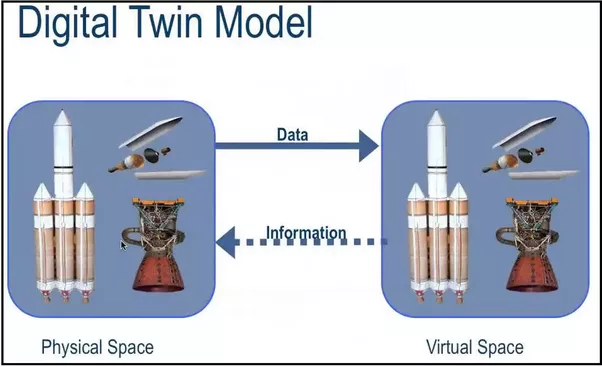
\includegraphics[scale=0.3]{images/digital_twin_auth.png} 
\vskip 1cm
%
%\begin{block}{Examples}
%Some examples of commonly used commands and features are included, to help you get started.
%\end{block}

\end{frame}
%%%%%%%%%%%%%%%%%%%%%%%%%%%%%%%%%%%%%%%%%%%%
\begin{frame}{Origine du jumeau numérique}
  \begin{itemize}
    \item Le concept a été introduit en 2003 lors d’un cours sur la gestion du cycle de vie des produits (PLM) à l'Université du Michigan par le Dr. Michael Grieves. Le Modèle numérique de ce Concept comme une mise en miroir de ce qui existe dans le monde réel et ce qui existe dans le monde virtuel.
    \item Le jumeau numérique a été déja adopté par la NASA comme base conceptuelle dans les domaines de l'astronautique et de l'aérospatiale depuis les années 70.
  \end{itemize}
\end{frame}
%%%%%%%%%%%%%%%%%%%%%%%%%%%%%%%%%%%%%%%%%%%%
\section{Gestion du cycle de vie des produits}

\subsection{Gestion du cycle de vie des produits}

\begin{frame}{Gestion du cycle de vie des produits}

\begin{itemize}
	\item Contester les conventions grâce à Digital Twin Concept et transformer fabrication.
	\item Processus en 6 étapes introduit à ce concept. 
\end{itemize}

% Commands to include a figure:
%\begin{figure}
%\includegraphics[width=\textwidth]{your-figure's-file-name}
%\caption{\label{fig:your-figure}Caption goes here.}
%\end{figure}

%\begin{table}
%\centering
%\begin{tabular}{l|r}
%Item & Quantity \\\hline
%Widgets & 42 \\
%Gadgets & 13
%\end{tabular}
%\caption{\label{tab:widgets}An example table.}
%\end{table}

\end{frame}
%%%%%%%%%%%%%%%%%%%%%%%%%%%%%%%%%%%%%%%%%%%%
\subsection{Exemples}

\begin{frame}{Exemples}

\begin{columns}[T] % align columns
\begin{column}{.38\textwidth}
\begin{itemize}
   \item Une voiture F1 est surveillée en temps réel avec de nombreux capteurs afin que l’équipage des stands puisse modifier les paramètres, demander au pilote de ralentir ou de modifier son comportement sur la piste si nécessaire.
   \item Industrie pharmaceutique, .
   \item Un jumeau numérique peut d'un bras de robot peut être utilisé par un chirurgien pour effectuer une opération à distance.
 \end{itemize}
\end{column}%
\hfill%
\begin{column}{.48\textwidth}
%\includegraphics[scale=0.6]{images/OKI-2.jpg} 
\end{column}%
\end{columns}
\end{frame}
%%%%%%%%%%%%%%%%%%%%%%%%%%%%%%%%%%%%%%%%%%%%
\subsection{Différence entre l'IoT et le jumeau numérique}
\begin{frame}{Différence entre l'IoT et les jumeaux numériques}
 \begin{itemize}
  \item Pour l'IoT, on aspire des data d'un objet physique et son environnement grâce à des capteurs, 
  \item Pour le digital twin, on injecte de la donnée dans un objet virtuel, que l'on fait évoluer au fur et à mesure de son vieillissement.
  \item Sans \textcolor{red}{capteur}, le Digital Twin ne peuvent pas exister!.
 \end{itemize}
\end{frame}
%%%%%%%%%%%%%%%%%%%%%%%%%%%%%%%%%%%%%%%%%%%%
\subsection{Différence entre la simulation et le jumeau numérique}
\begin{frame}{ Différence entre la simulation et les jumeaux numériques}
 \begin{itemize}
   \item Une plate-forme rassemble tous les experts pour fournir des analyses, des informations et des 
   diagnostics puissants.
 \end{itemize}
\end{frame}
%%%%%%%%%%%%%%%%%%%%%%%%%%%%%%%%%%%%%%%%%%%%
  \section{Définition formelle et ses types}
   \subsection{Définition formelle et ses types}
 \begin{frame}{Définition formelle et ses types}
   \begin{itemize}
     \item Digital Twin est un ensemble de constructions d'informations virtuelles qui décrit de manière complète un produit fabriqué physique ou potentiel, du niveau micro-atomique au niveau macro-géométrique. À son optimum, toute information pouvant être obtenue auprès de l’inspection d’un produit physique fabriqué peut être obtenue auprès de son Digital Twin.
     \item Les jumeaux numériques sont de deux types:
       \begin{itemize}
         \item Digital Prototype Twin (DTP)
         \item Instance numérique double (DTI)
       \end{itemize}
     \item Les DT sont utilisés dans un environnement double numérique (DTE).
   \end{itemize}
  \end{frame}
%%%%%%%%%%%%%%%%%%%%%%%%%%%%%%%%%%%%%%%%%%%%
 \begin{frame}{Tyes}
   \begin{itemize}
     \item Digital Prototype Twin (DTP).
     \item Instance numérique double (DTI).
     \item Digital Twin Aggregate (DTA).
   \end{itemize}
  \end{frame}
%%%%%%%%%%%%%%%%%%%%%%%%%%%%%%%%%%%%%%%%%%%%%
  \begin{frame}{Objectif(s)}
   \begin{itemize}
     \item Digital Twin Environment (DTE) - C’est un environnement intégré, espace d'application physique multi-domaines pour l'exploitation de Digital Twins à diverses fins.
     \item Prédictif/préventif.
     \item Interrogatif
   \end{itemize}
  \end{frame}
 %%%%
 \begin{frame}{créer un jumeau numérique: comment ça marche?}
  La création d'un digital twin suit une démarche inverse:
    \begin{enumerate}
      \item on part d'une machine qui existe, sur laquelle on pose des capteurs, puis on dessine en 3D les éléments 
   qui nous semblent les plus critiques.
      \item  Si une partie de la machine n'a pas d'intérêt, elle n'a pas besoin d'être reproduite.
    \end{enumerate} 
 \end{frame}
 %%
 \begin{frame}{Cas d'utilisation d'un modèle jumeau numérique}
	 \begin{itemize}
       \item Risques pour la sécurité - Un moteur d'avion.
       \item Maintenance-A moteur de voiture de course.
       \item Assemblage - Un jumeau numérique d'une unité de climatisation.
       \item Smart City - comprend les structures souterraines telles que les systèmes d'eau.
       \item Testing-Un jumeau numérique d'un téléphone intelligent.
       \item Design- Imprimante 3D.
       \item Toute entité physique.
       \item Expérience client - modéliser les modes sur un jumeau visuel d'un client.
       \item PLM: la principale raison de sa création.
	 \end{itemize}
 \end{frame}
  %%%%%	 
  \begin{frame}{Portée}
  \begin{itemize}
      \item L'évolutivité..
      \item Humanoïde.
      \item Approche complètement 3D.
	  \item Interfaces et cartes.
  \end{itemize}
 \end{frame}
 %%%%%
 \begin{frame}{Quelques désavantages}
  \begin{itemize}
	  \item Mise en place coûteuse dans un cadre d'une industrie 4.0.
	  \item Dépendant de la connectivité internet.
	  \item La sécurité est en jeu.
      \item 39\% des travaux de conception produisent des dessins 2D, 27\% des modèles 3D et 34\% des dessins 
      2D. dessins et modèles 3D. Dessins 2D générés automatiquement à partir de CAO 3D les modèles sont 
      importants car il y a plus de développement logiciel sur le dessin 2D aptitude.
	 \item Le concept Digital Twin est basé sur des modèles CAO 3D et non sur des dessins 2D.
     \item Un jumeau numérique sera nécessaire pour toutes les chaînes d'approvisionnement.
     \item Les défis ici concernent la mondialisation et les nouvelles techniques de fabrication. Gérer toutes 
     ces données de conception pour le jumelage numérique entre partenaires et fournisseurs, le produit physique 
     évoluera sera un défi.
  \end{itemize}
 \end{frame}
 %%%%%

 %%%%%
 \begin{frame}{Pourquoi le Jumeau Numérique peut etre si important pour le libre?}
  \begin{itemize}
	\item C'est toujours bénéfique. et sa peut aboutir à un autre idée. 	
	\item Un pont entre le libre et l'industrie 4.0.
	\item Comment les projets et les communautés libres, bénéficie t-elle du jumeau numérique.
	\item PLM Libre/Open Source, redéfinir et crée de nouveaux concepts.
  \end{itemize}
 \end{frame}
 %%%%%
 %%%%%
 \begin{frame}{Questions ?}
 Questions ?
  \end{frame}
%%%%%%%%%
 \begin{frame}{Fin}
	 \center{Questions ?}
 \end{frame}
\end{document}
